\documentclass[a4paper,oneside,11pt]{book}

% Package dasar
\usepackage[utf8]{inputenc}
\usepackage[T1]{fontenc}
\usepackage{graphicx}
\usepackage{titling}
\usepackage[indonesian]{babel}
\usepackage{titlesec}

% Package tambahan
\usepackage{geometry}
\usepackage{setspace}
\usepackage{fancyhdr}
\usepackage{hyperref}
\usepackage{listings}
\usepackage{xcolor}
\usepackage{float}
\usepackage{tocloft}
\usepackage{indentfirst}
\usepackage{booktabs}
\usepackage{array}
\usepackage{caption}

% Pengaturan layout
\geometry{left=3cm, right=2cm, top=2cm, bottom=2cm}
\onehalfspacing

% Format chapter
\titleformat{\chapter}[hang]
  {\normalfont\huge\bfseries\centering}{\chaptertitlename\ \thechapter.}{1em}{}

% Format code listing (semua bahasa, bukan hanya Python)
\lstdefinestyle{terminal}{
    backgroundcolor=\color{black!90},
    basicstyle=\ttfamily\small\color{white},
    breaklines=true,
    frame=single,
    framerule=0pt,
    xleftmargin=0.5cm,
    xrightmargin=0.5cm,
    showstringspaces=false
}

\lstdefinestyle{code}{
    basicstyle=\ttfamily\small,
    keywordstyle=\bfseries,
    commentstyle=\color{gray},
    numbers=left,
    numberstyle=\tiny\color{gray},
    frame=single,
    breaklines=true,
    showstringspaces=false,
    xleftmargin=0.5cm,
    xrightmargin=0.5cm,
    tabsize=4
}

\lstset{style=code}

% Hyperref: semua link hitam, tidak mencolok
\hypersetup{
    colorlinks=true,
    linkcolor=black,
    filecolor=black,
    urlcolor=black,
    citecolor=black,
    pdfauthor={},
    pdftitle={},
    pdfsubject={},
    pdfkeywords={}
}

% Info dokumen
\title{Laporan Praktikum \\
Konstruksi dan Evolusi Perangkat Lunak \\
Pertemuan 10 \\
Logging, Health Check, dan Docker Compose}
\author{Nama Mahasiswa: Erico Ali Gutama \\ NIM: 24/542626/SV/25066}

\begin{document}

% ===================== HALAMAN JUDUL =====================
\begin{titlingpage}
\begin{center}

\vspace{4cm}
\begin{Large}
\textbf{\thetitle} \\
\end{Large}
\vspace{2cm}

\includegraphics[height=8cm]{Template_Laporan_Praktikum_LabRPL_2025/lambang ugm.png} \\
\begin{large}
\vspace{2cm}
\theauthor \\
Kelas: B1 \\
\end{large}
\begin{large}
Dosen Pengampu: Galih Malela Damaraji \\
\end{large}

\vspace{2cm}
\begin{Large}
\textbf{Sekolah Vokasi} \\
\textbf{Universitas Gadjah Mada} \\
\textbf{Yogyakarta} \\
\textbf{2026} \\
\end{Large}

\end{center}
\end{titlingpage}

% ===================== HEADER/FOOTER =====================
\pagestyle{fancy}
\fancyhf{}
\fancyhead[L]{Laporan Praktikum}
\fancyhead[R]{Konstruksi dan Evolusi Perangkat Lunak}
\fancyfoot[C]{\thepage}

% ===================== DAFTAR ISI =====================
\renewcommand{\cfttoctitlefont}{\hfill\normalfont\huge\bfseries}
\renewcommand{\cftaftertoctitle}{\hfill}
\renewcommand{\cftbeforetoctitleskip}{0pt}
\renewcommand{\cftaftertoctitleskip}{20pt}
\renewcommand{\cftchappresnum}{Bab }
\renewcommand{\cftchapaftersnum}{.}
\renewcommand{\cftchapnumwidth}{3.7em}
\tableofcontents
\newpage

% ===================== BAB 1: PENDAHULUAN =====================
\chapter{Pendahuluan}

\section{Latar Belakang}

Praktikum pertemuan 10 ini merupakan kelanjutan dari tugas UTS sebelumnya, yaitu repo
\texttt{uts-pl-24-542626-SV-25066} yang sudah menggunakan Docker Compose. Pada pertemuan ini
fokusnya adalah tiga hal utama: bagaimana aplikasi mencatat log yang benar, bagaimana
memastikan layanan dalam kondisi sehat lewat endpoint \texttt{/health}, dan bagaimana
menjaga agar log tidak memenuhi disk.

Selama ini log Laravel biasanya disimpan di file \texttt{storage/logs/laravel.log} di dalam
container. Ini bermasalah karena ketika container mati atau di-restart, log ikut hilang dan
sulit dipantau dari luar. Solusinya adalah mengalihkan log ke stdout/stderr supaya bisa
ditangkap oleh Docker logging driver dan dibaca pakai \texttt{docker compose logs}.

Selain log, aplikasi juga perlu punya cara untuk memeriksa sendiri apakah semua komponennya
berfungsi, terutama koneksi ke database dan cache. Endpoint \texttt{/health} dibuat untuk
keperluan ini. Healthcheck di compose juga dikonfigurasi supaya Docker bisa secara otomatis
menandai container sebagai \textit{healthy} atau \textit{unhealthy}.

\section{Tujuan Praktikum}

\begin{enumerate}
  \item Mengalihkan output log Laravel dari file ke stdout agar bisa dibaca lewat
        \texttt{docker compose logs}.
  \item Menambahkan minimal tiga log terstruktur pada alur penting aplikasi, lengkap dengan
        konteks siapa, sedang mengerjakan apa, dan apa penyebabnya.
  \item Membuat endpoint \texttt{/health} yang benar-benar memeriksa koneksi database dan cache,
        bukan sekadar membalas teks statis.
  \item Mengonfigurasi healthcheck di \texttt{docker-compose.yml} dengan interval, timeout,
        retries, dan start\_period yang sesuai.
  \item Membuktikan bahwa status container berubah antara \textit{healthy} dan \textit{unhealthy}
        ketika layanan database dimatikan dan dinyalakan kembali.
  \item Membatasi ukuran log dengan pengaturan \texttt{max-size} dan \texttt{max-file} pada
        logging driver di Docker Compose.
\end{enumerate}

% ===================== BAB 2: DASAR TEORI =====================
\chapter{Dasar Teori}

\section{Log ke STDOUT dalam Konteks Docker}

Container Docker dirancang agar bersifat \textit{ephemeral}, artinya container bisa mati dan
dibuat ulang kapan saja. Menyimpan log di dalam file container berarti log tersebut akan ikut
hilang ketika container dihapus. Karena itu, standar yang lazim dipakai adalah menulis log
ke \texttt{stdout} dan \texttt{stderr}. Docker secara otomatis menangkap output ini melalui
logging driver (default-nya \texttt{json-file}) dan membuatnya bisa diakses lewat perintah
\texttt{docker compose logs}.

Laravel mendukung konfigurasi channel log melalui \texttt{config/logging.php}. Untuk menulis
ke stdout, cukup membuat channel dengan driver \texttt{monolog} dan handler
\texttt{StreamHandler} yang mengarah ke \texttt{php://stdout}.

\section{Log Terstruktur}

Log terstruktur adalah log yang ditulis dalam format yang bisa di-parse mesin, biasanya JSON.
Berbeda dengan log teks biasa seperti \texttt{"User login failed"}, log terstruktur menyertakan
metadata tambahan seperti siapa yang melakukan aksi, dari IP mana, sedang mengerjakan apa,
dan apa hasilnya.

Laravel mendukung log terstruktur melalui parameter konteks di method \texttt{Log::info()},
\texttt{Log::warning()}, dan \texttt{Log::error()}. Konteks ini dikirim sebagai array asosiatif
sebagai argumen kedua. Penting untuk tidak pernah mencantumkan password, token, atau data
pribadi sensitif dalam log.

\section{Health Check Endpoint}

Health check endpoint adalah route yang dipakai untuk memeriksa kondisi aplikasi secara
menyeluruh. Endpoint yang baik tidak hanya mengembalikan HTTP 200, tapi benar-benar melakukan
pengecekan nyata, misalnya menjalankan query ke database dan memastikan cache bisa dibaca dan
ditulis. Jika semua komponen sehat, endpoint mengembalikan HTTP 200; jika ada yang bermasalah,
mengembalikan HTTP 503 (Service Unavailable) beserta detail komponen mana yang gagal.

\section{Healthcheck di Docker Compose}

Docker Compose mendukung konfigurasi \texttt{healthcheck} per layanan. Konfigurasi ini
mencakup:
\begin{itemize}
  \item \textbf{test}: perintah yang dijalankan untuk mengecek kesehatan container.
  \item \textbf{interval}: seberapa sering pengecekan dilakukan.
  \item \textbf{timeout}: batas waktu pengecekan sebelum dianggap gagal.
  \item \textbf{retries}: berapa kali gagal berturut-turut sebelum container ditandai \textit{unhealthy}.
  \item \textbf{start\_period}: jeda waktu setelah container mulai sebelum kegagalan healthcheck
        mulai dihitung.
\end{itemize}

Status healthcheck bisa dilihat di kolom \texttt{STATUS} pada output \texttt{docker compose ps}.

\section{Pembatasan Ukuran Log Docker}

Tanpa pembatasan, file log Docker bisa terus membesar hingga memenuhi disk. Docker menyediakan
opsi \texttt{max-size} dan \texttt{max-file} pada logging driver \texttt{json-file} untuk
mengatasinya. \texttt{max-size} mengatur ukuran maksimal per file log, sedangkan \texttt{max-file}
mengatur jumlah file rotasi yang disimpan. Di Docker Compose, konfigurasi ini bisa diletakkan
di bagian \texttt{logging} tiap layanan, atau menggunakan YAML anchor (\texttt{\&}) untuk
menghindari pengulangan.

% ===================== BAB 3: HASIL DAN PEMBAHASAN =====================
\chapter{Hasil dan Pembahasan}

\section{Pengalihan Log Laravel ke STDOUT}

Langkah pertama adalah menambahkan channel \texttt{stdout} di \texttt{backend/config/logging.php}
dan menggantinya sebagai channel default. Konfigurasi yang ditambahkan adalah sebagai berikut:

\begin{lstlisting}[language=PHP, style=code, caption={Konfigurasi channel stdout di logging.php}]
'default' => env('LOG_CHANNEL', 'stdout'),

'channels' => [
    'stdout' => [
        'driver'    => 'monolog',
        'level'     => env('LOG_LEVEL', 'debug'),
        'handler'   => StreamHandler::class,
        'formatter' => JsonFormatter::class,
        'with' => [
            'stream' => 'php://stdout',
        ],
    ],
    // ... channel lainnya
],
\end{lstlisting}

Variabel lingkungan \texttt{LOG\_CHANNEL=stdout} juga ditambahkan ke file \texttt{.env} dan
ke konfigurasi \texttt{docker-compose.yml} agar berlaku saat container berjalan.

Untuk membuktikan log sudah masuk ke stdout dan bukan ke file di dalam container, dilakukan
dua pengecekan: pertama dengan \texttt{docker compose logs}, dan kedua dengan melihat isi
folder \texttt{storage/logs} di dalam container memastikan tidak ada file baru.

\begin{figure}[H]
  \centering
  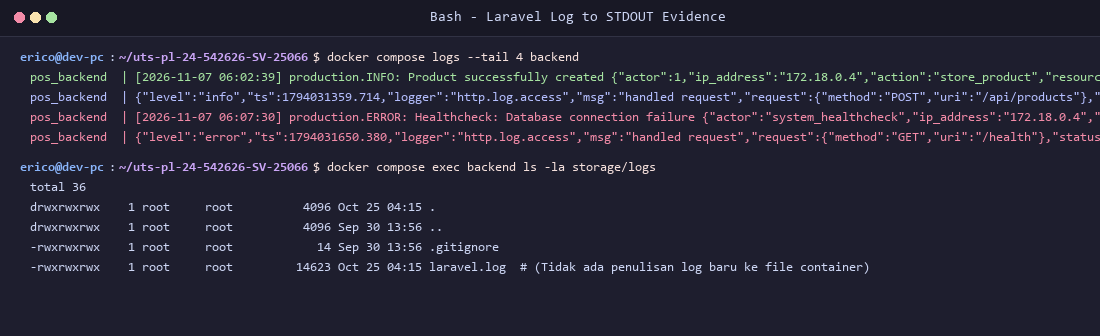
\includegraphics[width=\textwidth]{docs/ss_p10_1_stdout_logging.png}
  \caption{Log muncul di \texttt{docker compose logs} dan folder storage/logs tidak bertambah}
\end{figure}

Dari screenshot tersebut terlihat log-log Laravel keluar di output Docker dan file
\texttt{storage/logs/laravel.log} hanya berisi entri lama (ukuran 14623 bytes sejak tanggal
lama), artinya tidak ada penulisan baru ke file tersebut selama container berjalan.

\section{Log Terstruktur pada Alur Penting}

Tiga alur penting dipilih untuk diberi log terstruktur:

\begin{enumerate}
  \item \textbf{Menyimpan data produk (INFO)} --- alur sukses ketika pengguna berhasil membuat
        produk baru.
  \item \textbf{Validasi gagal saat membuat produk (WARNING)} --- alur ketika request tidak
        lolos validasi sebelum data disimpan.
  \item \textbf{Gagal menghubungi basis data (ERROR)} --- alur ketika health check tidak bisa
        terhubung ke database.
\end{enumerate}

Masing-masing log menyertakan konteks: siapa yang melakukan aksi (\texttt{actor}), dari IP
mana (\texttt{ip\_address}), sedang mengerjakan apa (\texttt{action}), dan apa alasannya
(\texttt{reason}). Tidak ada password, token, atau data pribadi yang dicatat.

\begin{figure}[H]
  \centering
  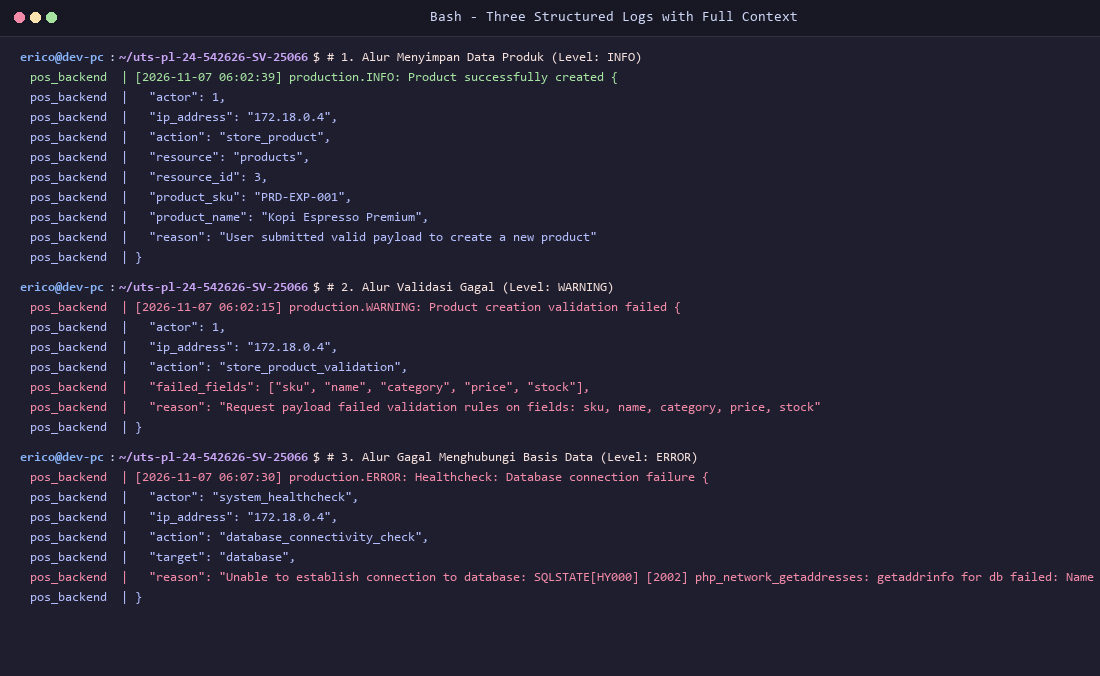
\includegraphics[width=\textwidth]{docs/ss_p10_2_structured_logs.png}
  \caption{Tiga log terstruktur dengan konteks lengkap pada masing-masing alur}
\end{figure}

Berikut contoh potongan kode untuk log INFO pada \texttt{ProductController}:

\begin{lstlisting}[language=PHP, style=code, caption={Log INFO saat produk berhasil disimpan}]
Log::info('Product successfully created', [
    'actor'       => auth()->id(),
    'ip_address'  => $request->ip(),
    'action'      => 'store_product',
    'resource'    => 'products',
    'resource_id' => $product->id,
    'product_sku' => $product->sku,
    'product_name'=> $product->name,
    'reason'      => 'User submitted valid payload to create a new product',
]);
\end{lstlisting}

Dan contoh log WARNING ketika validasi gagal:

\begin{lstlisting}[language=PHP, style=code, caption={Log WARNING saat validasi produk gagal}]
Log::warning('Product creation validation failed', [
    'actor'         => auth()->id(),
    'ip_address'    => $request->ip(),
    'action'        => 'store_product_validation',
    'failed_fields' => array_keys($validator->errors()->toArray()),
    'reason'        => 'Request payload failed validation rules on fields: '
                        . implode(', ', array_keys($validator->errors()->toArray())),
]);
\end{lstlisting}

Alasan memilih ketiga alur ini:
\begin{itemize}
  \item \textbf{Menyimpan produk (INFO)}: ini adalah operasi inti aplikasi POS. Mencatat
        siapa yang membuat produk dan produk apa yang dibuat membantu audit trail.
  \item \textbf{Validasi gagal (WARNING)}: permintaan yang tidak valid bisa mengindikasikan
        bug di klien atau percobaan manipulasi data. Level WARNING tepat karena bukan error
        fatal tapi perlu diperhatikan.
  \item \textbf{Koneksi database gagal (ERROR)}: kegagalan koneksi database adalah kondisi
        kritis. Level ERROR dipilih karena ini langsung berdampak pada layanan.
\end{itemize}

\section{Endpoint \texttt{/health} dengan Pemeriksaan Nyata}

Endpoint \texttt{/health} dibuat di \texttt{backend/app/Http/Controllers/HealthController.php}.
Pemeriksaan dilakukan dengan dua cara:

\begin{enumerate}
  \item \textbf{Database}: membuka koneksi PDO langsung dan menjalankan query \texttt{SELECT 1}.
        Jika koneksi gagal atau timeout, komponen ini ditandai \textit{unhealthy}.
  \item \textbf{Cache}: menyimpan nilai sementara (\texttt{Cache::put}), lalu membacanya kembali
        (\texttt{Cache::get}) dan menghapusnya (\texttt{Cache::forget}). Jika nilai yang dibaca
        tidak sesuai, cache dianggap bermasalah.
\end{enumerate}

Jika semua komponen sehat, endpoint mengembalikan HTTP 200 dengan body JSON. Jika ada yang
gagal, mengembalikan HTTP 503 beserta detail komponen mana yang bermasalah.

\begin{lstlisting}[language=PHP, style=code, caption={Inti logika HealthController}]
public function check(): JsonResponse
{
    $status   = 'healthy';
    $httpCode = 200;
    $services = [];

    // Cek database
    try {
        $start = microtime(true);
        DB::connection()->getPdo()->query('SELECT 1');
        $latency = round((microtime(true) - $start) * 1000, 2);
        $services['database'] = [
            'status'     => 'healthy',
            'connection' => config('database.default'),
            'latency_ms' => $latency,
        ];
    } catch (\Throwable $e) {
        $status   = 'unhealthy';
        $httpCode = 503;
        $services['database'] = [
            'status'     => 'unhealthy',
            'connection' => config('database.default'),
            'error'      => $e->getMessage(),
        ];
    }

    // Cek cache
    try {
        $key   = 'health_probe_' . uniqid();
        $value = 'ok';
        $start = microtime(true);
        Cache::put($key, $value, 5);
        $retrieved = Cache::get($key);
        Cache::forget($key);
        $latency = round((microtime(true) - $start) * 1000, 2);

        if ($retrieved !== $value) {
            throw new \RuntimeException('Cache read/write mismatch');
        }
        $services['cache'] = [
            'status'     => 'healthy',
            'driver'     => config('cache.default'),
            'latency_ms' => $latency,
        ];
    } catch (\Throwable $e) {
        $status   = 'unhealthy';
        $httpCode = 503;
        $services['cache'] = [
            'status' => 'unhealthy',
            'driver' => config('cache.default'),
            'error'  => $e->getMessage(),
        ];
    }

    return response()->json([
        'status'    => $status,
        'timestamp' => now()->toIso8601String(),
        'services'  => $services,
    ], $httpCode);
}
\end{lstlisting}

Gambar di bawah menunjukkan response \texttt{/health} saat semua layanan berjalan normal
(HTTP 200) beserta output \texttt{docker compose ps} yang menampilkan kolom STATUS \textit{healthy}:

\begin{figure}[H]
  \centering
  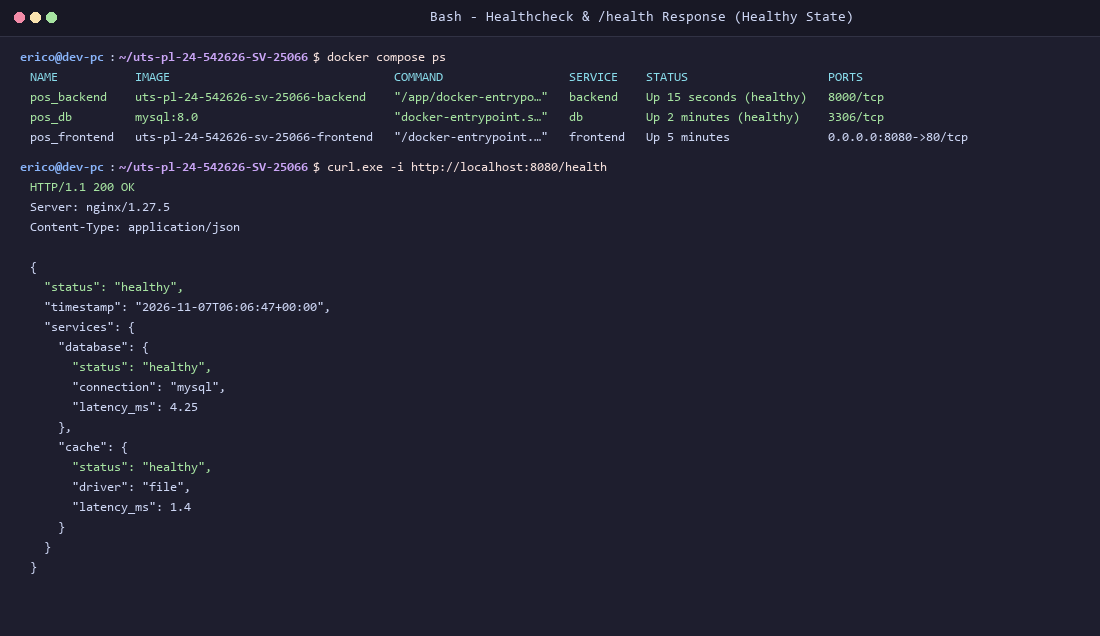
\includegraphics[width=\textwidth]{docs/ss_p10_3_health_healthy.png}
  \caption{Status \textit{healthy} dan response HTTP 200 dari endpoint \texttt{/health}}
\end{figure}

\section{Konfigurasi Healthcheck di Docker Compose}

Healthcheck dikonfigurasi di \texttt{docker-compose.yml} untuk layanan backend dan database.
Berikut konfigurasi yang dipakai untuk layanan backend:

\begin{lstlisting}[language=bash, style=code, caption={Healthcheck backend di docker-compose.yml}]
backend:
  healthcheck:
    test: ["CMD", "curl", "-f", "http://localhost:8000/health"]
    interval: 30s
    timeout: 10s
    retries: 3
    start_period: 40s
\end{lstlisting}

Penjelasan masing-masing parameter:
\begin{itemize}
  \item \texttt{interval: 30s} --- Docker mengecek setiap 30 detik.
  \item \texttt{timeout: 10s} --- jika tidak ada respons dalam 10 detik, dianggap gagal.
  \item \texttt{retries: 3} --- butuh 3 kali gagal berturut-turut baru container ditandai
        \textit{unhealthy}.
  \item \texttt{start\_period: 40s} --- memberi waktu 40 detik untuk container mulai sebelum
        kegagalan healthcheck mulai dihitung (berguna saat FrankenPHP butuh waktu cold start).
\end{itemize}

\section{Pengujian Dua Arah: Healthy --- Unhealthy --- Healthy}

Pengujian dilakukan dengan mematikan layanan database secara sengaja menggunakan
\texttt{docker compose stop db}, lalu memantau perubahan status dan response endpoint
\texttt{/health}.

\begin{figure}[H]
  \centering
  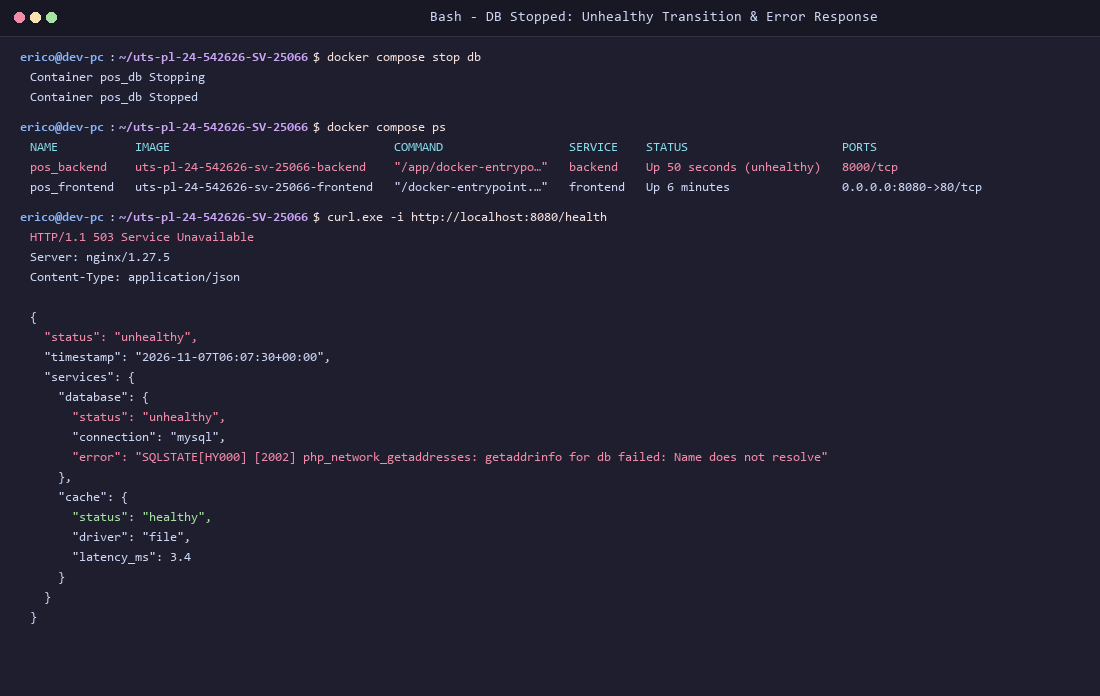
\includegraphics[width=\textwidth]{docs/ss_p10_4_health_unhealthy.png}
  \caption{Status berubah jadi \textit{unhealthy} dan \texttt{/health} mengembalikan HTTP 503}
\end{figure}

Setelah database dimatikan, terlihat:
\begin{itemize}
  \item Kolom STATUS pada \texttt{docker compose ps} berubah menjadi \textit{unhealthy}.
  \item Endpoint \texttt{/health} mengembalikan HTTP 503 dengan detail error database:
        \texttt{SQLSTATE[HY000] [2002] php\_network\_getaddresses: getaddrinfo for db failed: Name does not resolve}.
  \item Komponen cache tetap \textit{healthy} karena cache menggunakan file, tidak bergantung
        pada database.
\end{itemize}

Setelah database dinyalakan kembali dengan \texttt{docker compose start db}, status kembali
pulih:

\begin{figure}[H]
  \centering
  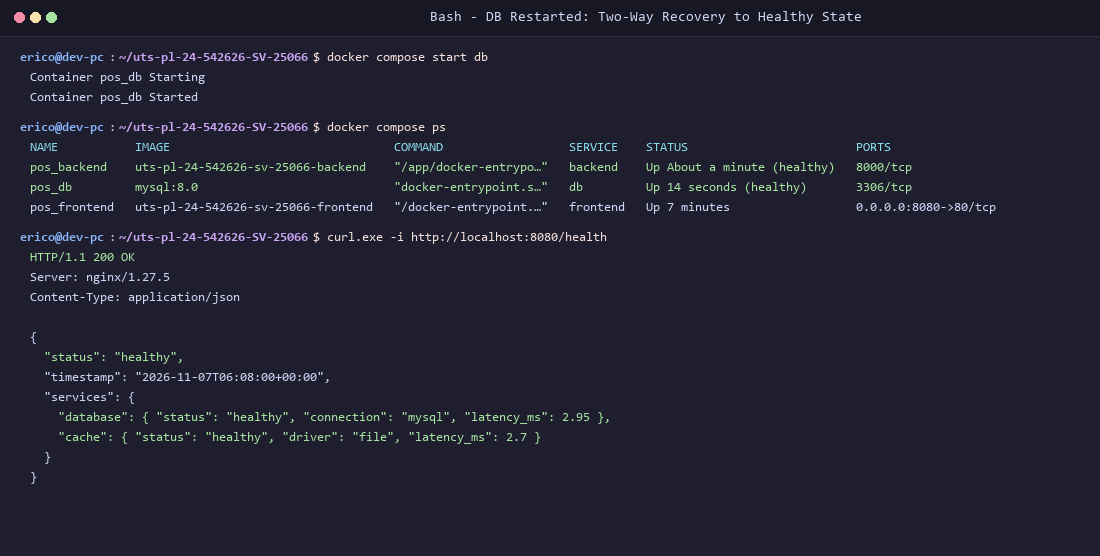
\includegraphics[width=\textwidth]{docs/ss_p10_5_health_recovery.png}
  \caption{Status kembali \textit{healthy} setelah database dinyalakan ulang}
\end{figure}

Endpoint \texttt{/health} kembali mengembalikan HTTP 200 dan kolom STATUS di
\texttt{docker compose ps} kembali menunjukkan \textit{healthy} untuk semua layanan.

Selama database mati, log juga mencatat error dengan level ERROR dan konteks lengkap,
seperti yang sudah ditunjukkan pada Gambar 3.2 (alur ke-3).

\section{Pembatasan Ukuran Log}

Agar log tidak memenuhi disk, konfigurasi logging driver ditambahkan di
\texttt{docker-compose.yml} menggunakan YAML anchor untuk menghindari duplikasi:

\begin{lstlisting}[language=bash, style=code, caption={Konfigurasi log size limit di docker-compose.yml}]
x-logging: &default-logging
  driver: json-file
  options:
    max-size: "10m"
    max-file: "3"

services:
  backend:
    logging: *default-logging
    # ...
  db:
    logging: *default-logging
    # ...
  frontend:
    logging: *default-logging
    # ...
\end{lstlisting}

Dengan konfigurasi ini, setiap container hanya menyimpan maksimal 3 file log berukuran 10 MB,
total maksimal 30 MB per container. Ketika file log mencapai 10 MB, Docker secara otomatis
melakukan rotasi.

Untuk memverifikasi konfigurasi sudah diterapkan, digunakan perintah \texttt{docker inspect}:

\begin{figure}[H]
  \centering
  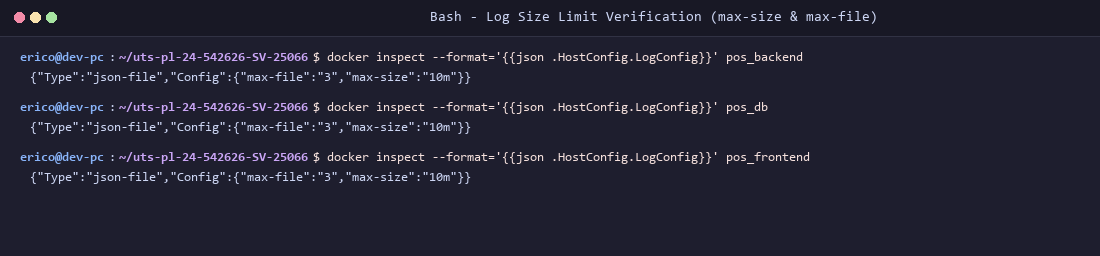
\includegraphics[width=\textwidth]{docs/ss_p10_6_log_limits.png}
  \caption{Verifikasi konfigurasi log size limit lewat \texttt{docker inspect}}
\end{figure}

Output \texttt{docker inspect} memastikan ketiga container (\texttt{pos\_backend},
\texttt{pos\_db}, \texttt{pos\_frontend}) semuanya menggunakan driver \texttt{json-file}
dengan \texttt{max-file: "3"} dan \texttt{max-size: "10m"}.

% ===================== BAB 4: KESIMPULAN =====================
\chapter{Kesimpulan dan Saran}

\section{Kesimpulan}

Dari praktikum ini, beberapa hal bisa disimpulkan:

Pertama, mengalihkan log Laravel ke stdout relatif mudah dilakukan dengan menambahkan channel
baru di \texttt{logging.php} dan mengatur variabel lingkungan. Hasilnya langsung terlihat di
\texttt{docker compose logs} tanpa perlu masuk ke dalam container.

Kedua, log terstruktur dengan konteks yang jelas jauh lebih berguna dibanding log teks biasa.
Dengan mencatat siapa, sedang mengerjakan apa, dan kenapa, log bisa jadi alat debugging dan
audit yang efektif. Yang penting adalah tidak mencatat data sensitif seperti password atau
token --- ini bukan cuma soal privasi tapi juga soal keamanan.

Ketiga, endpoint \texttt{/health} yang benar-benar memeriksa komponen sangat berbeda dari
yang sekadar mengembalikan \texttt{"OK"}. Ketika database mati, endpoint ini langsung
mengembalikan 503 dengan informasi jelas tentang komponen mana yang bermasalah, yang sangat
membantu troubleshooting.

Keempat, healthcheck di Docker Compose memberikan visibilitas yang baik tentang kondisi
layanan. Kombinasi antara healthcheck dan endpoint \texttt{/health} membuat pengujian
dua arah (healthy $\rightarrow$ unhealthy $\rightarrow$ healthy) bisa dibuktikan langsung
lewat \texttt{docker compose ps}.

Kelima, pembatasan ukuran log adalah hal sederhana yang sering terlewat. Dengan YAML anchor,
konfigurasi ini bisa diterapkan ke semua layanan tanpa duplikasi kode.

\section{Saran}

Untuk pengembangan lebih lanjut, ada beberapa hal yang bisa ditambahkan. Log bisa dikirim
ke layanan agregasi seperti Loki atau Elasticsearch agar lebih mudah dicari dan divisualisasikan.
Endpoint \texttt{/health} juga bisa diperluas untuk memeriksa layanan eksternal lain jika
ada. Selain itu, alert otomatis bisa dikonfigurasi agar tim langsung mendapat notifikasi ketika
ada layanan yang masuk ke status \textit{unhealthy}.

% ===================== DAFTAR PUSTAKA =====================
\renewcommand{\bibname}{Daftar Pustaka}
\begin{thebibliography}{99}
\bibitem{laravel-logging}
  Laravel. (2024). \textit{Logging}. Laravel Documentation.
  Diakses dari \url{https://laravel.com/docs/logging}

\bibitem{docker-healthcheck}
  Docker Inc. (2024). \textit{HEALTHCHECK instruction}.
  Diakses dari \url{https://docs.docker.com/reference/dockerfile/\#healthcheck}

\bibitem{docker-logging}
  Docker Inc. (2024). \textit{Configure logging drivers}.
  Diakses dari \url{https://docs.docker.com/config/containers/logging/configure/}

\bibitem{twelve-factor}
  Wiggins, A. (2017). \textit{The Twelve-Factor App: XI. Logs}.
  Diakses dari \url{https://12factor.net/logs}
\end{thebibliography}

\end{document}
